\chapter{单车最优控制仿真}
\label{cha:exp}
在\ref{sec:solve}和\ref{sec:cc}节分别给出了单车在无约束、有约束状况下的最优控制求解方法。本章将给出一些算例,验证方法的正确性。由于无约束最优控制求解比较简单,将其放在有约束问题的求解中一并讨论,并加以比较。

本章的算例使用{\ttfamily Mathematica}进行仿真。与\ref{sec:cc}节的约定相同,本节也使用下标区分变量的含义以避免歧义:$t_0$表示进入控制区的时间,$t_\mathrm{m}$表示进入交汇区的时间。

\section{速度约束下的最优控制}
速度约束下的最优控制可由式\eqref{eq:num:vopt0}---\eqref{eq:num:vopt9}描述的优化问题给出。

\subsection{较大速度约束}
首先考虑速度约束很大,实际最高速度不会超过约束的情形。这种情况下,由式\eqref{eq:num:vopt0}---\eqref{eq:num:vopt9}解出的最优控制应该与式\eqref{eq:noc:array}解出的一致。参数设置如表\ref{tab:vbig:param}所示。
\begin{table}[htbp]
\centering
\caption{大速度约束仿真实验参数}
\label{tab:vbig:param}
\begin{tabular}{lll}
\toprule[1.5pt]
参数符号 & 参数含义 & 参数值 \\
\midrule[1pt]
$p_0$ & 初始位移 & $0$ \\
$L$($p_\mathrm{m}$) & 控制区长度(终点位移) & $\SI{600.0}{m}$ \\
$v_0$ & 初速度 & $\SI{10.0}{m\per s}$ \\
$v_\mathrm{d}$ & 期望速度 & $\SI{25.0}{m\per s}$ \\
$t_0$ & 初始时刻 & $0$ \\
$t_\mathrm{m}$ & 到达路口时刻 & $\SI{25.0}{s}$ \\
$v_{\max}$ & 速度限制 & $\SI{30.0}{m\per s}$ \\
\bottomrule[1.5pt]
\end{tabular}
\end{table}

在该设定下,直接求解式\ref{eq:noc:array}可得,$a=-0.1248$,$b=2.16$。加速度与速度随时间变化的函数图像分别如图\ref{fig:da}与\ref{fig:dv}。由图可见,最大速度没有超过$v_{\max}=\SI{30.0}{m\per s}$的限制。
\begin{figure}[htbp]
\centering
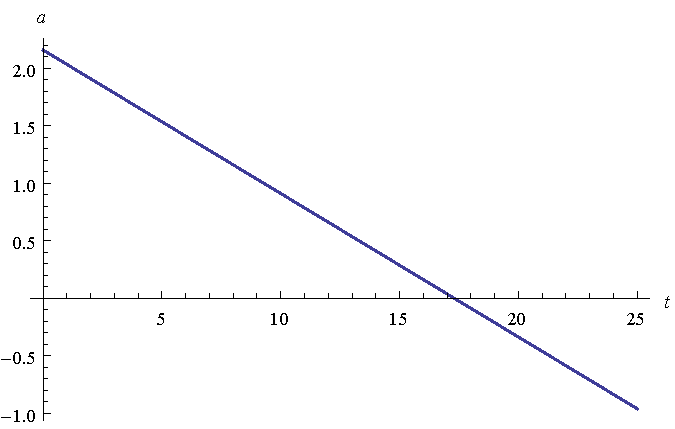
\includegraphics[width=9cm]{figures/vopt/da.pdf}
\caption{加速度理论解(大速度约束实验)}
\label{fig:da}
\end{figure}
\begin{figure}[htbp]
\centering
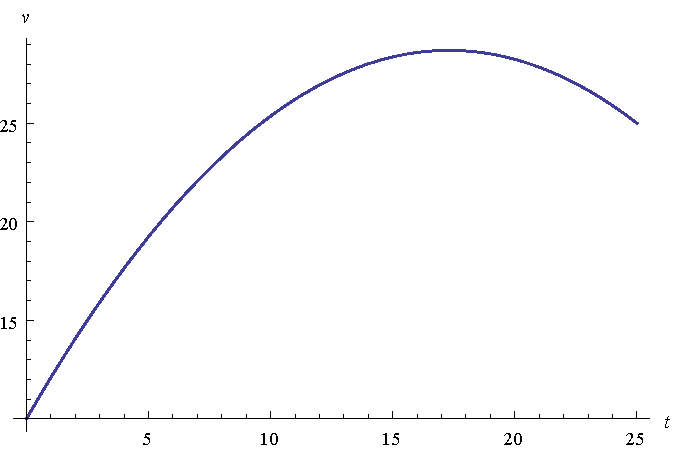
\includegraphics[width=9cm]{figures/vopt/dv.pdf}
\caption{速度理论解(大速度约束实验)}
\label{fig:dv}
\end{figure}

对于由式\eqref{eq:num:vopt0}---\eqref{eq:num:vopt9}确定的优化问题,使用 Nelder Mead 方法进行搜索,共做10次实验,得到的结果如表\ref{tab:vbig:res}。其中只有第3、9组收敛,第1、5、6、8组均不满足等式约束,第2、4、7、10组是因为数值运算产生了精度损失,导致目标函数接近零,实际不是可行解。
\begin{table}[htbp]
\centering
\caption{大速度约束仿真结果}
\label{tab:vbig:res}
\npdecimalsign{.}
\nprounddigits{2}
\definecolor{Gray}{gray}{0.85}
\newcolumntype{a}{>{\columncolor{Gray}}n{2}{2}}
\begin{tabular}{can{4}{2}n{3}{2}n{3}{2}n{3}{2}n{3}{2}n{2}{2}n{2}{2}}
\toprule[1.5pt]
组号 & \multicolumn{1}{c}{$2J$} & \multicolumn{1}{c}{$a_1$} & \multicolumn{1}{c}{$a_2$} & \multicolumn{1}{c}{$b_1$} & \multicolumn{1}{c}{$b_2$} & \multicolumn{1}{c}{$t_1$} & \multicolumn{1}{c}{$t_2$} & \multicolumn{1}{c}{$v_\mathrm{med}$} \\
\midrule[1pt]
1 & 31.9202 & -0.150847  & -1.25933 & 2.31784  & 28.9238  & 13.7106  & 22.9692  & 27.601 \\
2 & 0.947635 & 22.712 & -1.99535  & 0.161634  & 50.3226  & 0.102536  & 24.3986  & 25. \\
3 & 29.28 & -0.1248  & -0.1248  & 2.16  & 2.16  & 17.2988  & 17.3153  & 28.6923 \\
4 & 0.00210413 & -15.1761  & 5.19043  & 55.8682  & -67.2308  & 1.96593\text{e-7}  & 25.  & 26.6327 \\
5 & 28.7006 & -0.121663  & -0.68766  & 2.13381  & 17.186  & 25.039  & 25.  & 25.1455 \\
6 & 32.3924 & -0.156678  & -1.57797  & 2.35335  & 36.6386  & 13.5428  & 23.2196  & 27.5031 \\
7 & 0.00631779 & 2568.16  & -3.2169\text{e8}  & 1.37546\text{e5}  & -1.30641\text{e7}  & 3.33939\text{e-13}  & 25.  & 25. \\
8 & 32.087 & -0.152872  & -1.36605  & 2.3303  & 31.5039  & 13.6421  & 23.0634  & 27.565 \\
9 & 29.28 & -0.1248  & -0.1248  & 2.16  & 2.16  & 17.2996  & 17.3139  & 28.6923 \\
10 & 0.995235 & 34.6232  & 11.9513  & -0.0831005  & -380.425  & 0.136113  & 25.  & 25. \\
\bottomrule[1.5pt]
\end{tabular}
\end{table}

由获得的解可以看出,在速度约束不足以制约最优控制时,按照式\eqref{eq:num:vopt0}---\eqref{eq:num:vopt9}得到的解十分接近直接求解\eqref{eq:noc:array}得到的最优控制。作出仿真得到的加速度和速度函数图像,可以观察到与图\ref{fig:da}和图\ref{fig:dv}基本一样。这从一定程度上验证了优化问题(式\eqref{eq:num:vopt0}---\eqref{eq:num:vopt9})的正确性。

\subsection{较小速度约束}
在速度约束小的情形下,车辆为了保证在$t_\mathrm{m}$时间运行$L$位移,必须达到最大速度(按照优化问题提出的形式,保持某一小于最大速度的速度值也是可能的)并产生匀速运行段。下面的算例即为这种情况。参数设置如表\ref{tab:vsmall:param}所示。
\begin{table}[htbp]
\centering
\caption{小速度约束仿真实验参数}
\label{tab:vsmall:param}
\begin{tabular}{lll}
\toprule[1.5pt]
参数符号 & 参数含义 & 参数值 \\
\midrule[1pt]
$p_0$ & 初始位移 & $0$ \\
$L$($p_\mathrm{m}$) & 控制区长度(终点位移) & $\SI{700.0}{m}$ \\
$v_0$ & 初速度 & $\SI{10.0}{m\per s}$ \\
$v_\mathrm{d}$ & 期望速度 & $\SI{25.0}{m\per s}$ \\
$t_0$ & 初始时刻 & $0$ \\
$t_\mathrm{m}$ & 到达路口时刻 & $\SI{25.0}{s}$ \\
$v_{\max}$ & 最大速度限制 & $\SI{30.0}{m\per s}$ \\
\bottomrule[1.5pt]
\end{tabular}
\end{table}

在该设定下,直接求解式\ref{eq:noc:array}可得,$a=-0.2016$,$b=3.12$。加速度与速度随时间变化的函数图像分别如图\ref{fig:na}与\ref{fig:nv}。由图可见,最大速度已经超过了$v_{\max}=\SI{30.0}{m\per s}$的限制。
\begin{figure}[htbp]
\centering
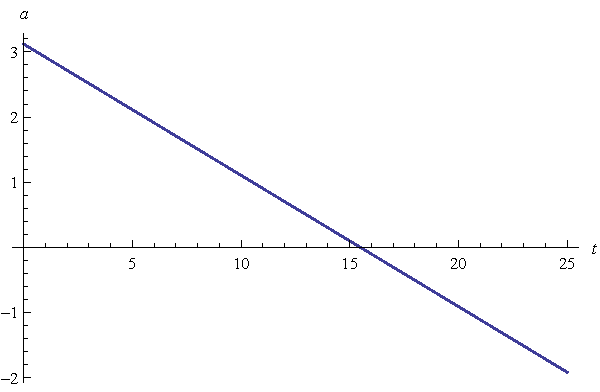
\includegraphics[width=9cm]{figures/vopt/na.pdf}
\caption{加速度理论解(小速度约束实验)}
\label{fig:na}
\end{figure}
\begin{figure}[htbp]
\centering
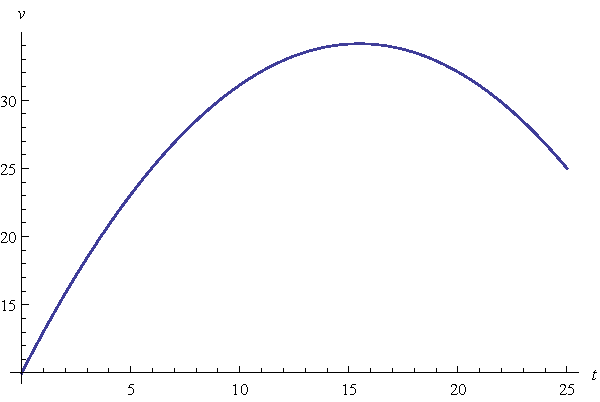
\includegraphics[width=9cm]{figures/vopt/nv.pdf}
\caption{速度理论解(小速度约束实验)}
\label{fig:nv}
\end{figure}

使用 Nelder Mead 方法进行搜索,共做10次实验,得到的结果如表\ref{tab:vsmall:res}。10组解中的第1,3,4,6,8,9组的目标函数都在$90.0$附近,第2,5,7组已经发散,第10组实验是因为$t_1$,$t_2$ 从中选取目标函数$J$最小的第二组验证约束,容易验证该组值满足所有约束条件。其加速度与速度的仿真结果如图\ref{fig:sa}与\ref{fig:sv}。
\begin{table}[htbp]
\centering
\caption{小速度约束仿真结果}
\label{tab:vsmall:res}
\npdecimalsign{.}
\nprounddigits{2}
\definecolor{Gray}{gray}{0.85}
\newcolumntype{a}{>{\columncolor{Gray}}n{4}{2}}
\begin{tabular}{can{3}{3}n{3}{3}n{3}{3}n{4}{2}n{3}{3}n{3}{3}n{3}{3}}
\toprule[1.5pt]
组号 & \multicolumn{1}{c}{$2J$} & \multicolumn{1}{c}{$a_1$} & \multicolumn{1}{c}{$a_2$} & \multicolumn{1}{c}{$b_1$} & \multicolumn{1}{c}{$b_2$} & \multicolumn{1}{c}{$t_1$} & \multicolumn{1}{c}{$t_2$} & \multicolumn{1}{c}{$v_\mathrm{med}$} \\
\midrule[1pt]
1 & 90. & -0.9  & -0.9 & 6.  & 19.5 & 6.66639  & 21.6675 & 30. \\
2 & 510.122 & -6.22911 & -51.8806  & 16.6683 & 1216.05  & 1.57173 & 24.9561 & 28.5041 \\
3 & 90. & -0.899999 & -0.899998  & 6. & 19.4999  & 6.66314 & 21.67 & 30. \\
4 & 90.4282 & -0.926215 & -0.484871  & 6.09571 & 9.71891  & 6.22471 & 22.0284 & 30. \\
5 & 2108.67 & -3.19281 & -0.82022  & 115.579 & 12.7663  & 0.156782 & 24.5931 & 28.0816 \\
6 & 90.2578 & -0.869418  & -1.21736 & 5.89715  & 26.9451 & 6.78285  & 22.1459 & 29.9998 \\
7 & 1442.69 & -7.31254  & -31.6065 & 78.943  & 776.161 & 0.231792  & 24.557 & 28.1019 \\
8 & 90. & -0.899999 & -0.899998  & 6. & 19.5  & 6.66248 & 21.6704 & 30. \\
9 & 90. & -0.899999 & -0.899996  & 6. & 19.4999  & 6.66221 & 21.6712 & 30. \\
10 & 27.9248 & 29.2397 & 4.45632  & 6.21342 & -105.163  & 0.248771 & 24.9273  & 28.0866 \\
\bottomrule[1.5pt]
\end{tabular}
\end{table}

\begin{figure}[htbp]
\centering
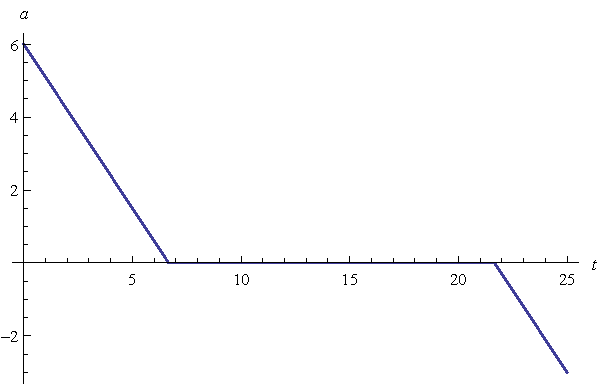
\includegraphics[width=9cm]{figures/vopt/sa.pdf}
\caption{小速度约束下加速度仿真结果}
\label{fig:sa}
\end{figure}
\begin{figure}[htbp]
\centering
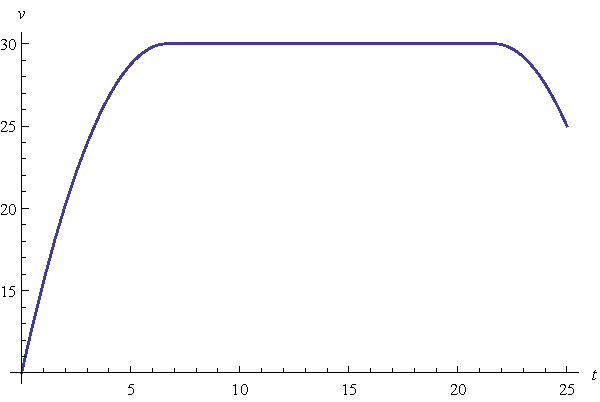
\includegraphics[width=9cm]{figures/vopt/sv.pdf}
\caption{小速度约束下速度仿真结果}
\label{fig:sv}
\end{figure}

由解得的最优控制可观察到如下特点:
\begin{enumerate}[label=(\arabic*)]
\item $v_\mathrm{med}=v_{\max}$,即匀速段速度值为最大速度;
\item $a_1=a_2$,即加速度段和减速段加速度的斜率相同;
\item $a_1(t_1)=a_2(t_2)=0$,即加速段的结束和减速段的开始时刻加速度均为0,加速度是连续的。
\end{enumerate}

这里不做证明地给出结论,在存在速度约束,且在式\eqref{eq:noc:array}的解超出速度限制的情况下,单个车辆的最优控制均有以上特点。这个结论可以理解为,将整个控制过程分为触发约束段和不触发约束段,所有不触发约束段拼接成完整的一段,应该等效于一个位移、时间都较短,无速度限制的最优控制问题,其加速度应该是一个完整的线性段。

\subsection{速度约束的简化问题}
基于以上的结论,可以进一步简化速度约束下最优控制问题的求解。以下按照之前解释的方法,将所有不触发约束段合成为一段,称为\textbf{变速段},中间匀速行驶的时段称为\textbf{匀速段}。假设变速段中加速度和速度表达式为
\begin{gather}
u(t)=at+b,\\
v(t)=\frac12at^2+bt+c,
\end{gather}
再设变速段持续时间为$t_\mathrm{c}$,并设$t_0=0$,$p_0=0$则可得方程组
\begin{gather}
v(0)=c=v_0,\label{eq:vopt:1}\\
v(t_\mathrm{c})=v_\mathrm{d},\\
v(-\frac ba)=v_\mathrm{m},\\
L-(t_\mathrm{m}-t_\mathrm{c})v_\mathrm{m}=\frac16at_\mathrm{c}^3+\frac12bt_\mathrm{c}^2+ct_\mathrm{c}.\label{eq:vopt:4}
\end{gather}
其中$v_\mathrm{m}$表示最大速度$v_{\max}$。该方程组有$a$,$b$,$c$与 $t_\mathrm{c}$四个待定参数。一般数值计算软件能够很快解出以上方程组,求得$t_\mathrm{c}$,$a$与$b$的值。则实际最优控制为
\begin{equation}
u^*(t)=
\begin{dcases}
at+b,\quad & t_0<t<t_0-\frac ba\ \text{ and}\\
\quad & t_\mathrm{m}-t_\mathrm{c}-\frac ab\leq t\leq t_\mathrm{m},\\
0,\quad & t_0-\frac ab \leq t < t_\mathrm{m}-t_\mathrm{c}-\frac ab.
\end{dcases}
\end{equation}
上式有一组实数解满足$2at_\mathrm{c}+b=0$,这组解在整个变速段加速度不变号,予以排除即可。

另外值得注意的是,上式在一定的参数范围内才适用。考虑两端的极限情况(设$t_0=0$,$p_0=0$):
\begin{enumerate}[label=(\arabic*)]
\item 一直以最大速度运行,则有
\begin{equation}
v_\mathrm{m}t_\mathrm{m}=L.\\
\end{equation}
\item 匀速段时间恰好为零,此时应满足(推导略),
\begin{gather}
\frac12at^2+bt+v_0=v_\mathrm{d},\\
\frac16at^3+\frac12bt^2+v_0t=L,\\
-\frac{b^2}{2a}+v_0=v_\mathrm{m}.
\end{gather}
\end{enumerate}
实际计算单个车辆具有速度限制的最优控制时,按照算法\ref{alg:vsin}求解。
\begin{algorithm}
\caption{速度限制下的单车最优控制求解}
\label{alg:vsin}
\begin{algorithmic}
  \Require{设$t_0=0$,$p_0=0$}
  \Statex
  \Function{GetOptimalControl}{$t_\mathrm{m},L,v_0,v_\mathrm{d}$}
    \If{$t_\mathrm{m} v_{\max}<=L$}
      \State $t_\mathrm{m}$计算错误
      \State \Return
    \EndIf
    \State 解\eqref{eq:noc:array},得到$u_1^*(t),v^*_1(t)$
    \If{$\max_t\{v^*_1(t)\}>v_{\max}$}
      \State 解\eqref{eq:vopt:1}---\eqref{eq:num:vopt4},得到$u_2^*(t),v^*_2(t)$
      \State \Return $u_2^*(t)$
    \Else
      \State \Return $u_1^*(t)$
    \EndIf
  \EndFunction
\end{algorithmic}
\end{algorithm}

\section{速度与加速度约束下的最优控制}
在速度与加速度约束同时存在时,直接优化式\eqref{eq:num:aopt1}---\eqref{eq:num:aoptL}参数太多,很难得到全局最优。而在上一节中,利用速度约束下最优控制的性质,可以将优化问题进一步简化为方程的求解。将简化的依据总结为引理\ref{lem:1},
\begin{lemma}
速度、加速度受限制的单车最优控制问题中,加速度最优解是连续的,且所有线性段具有相同的斜率。
\label{lem:1}
\end{lemma}
引理的证明略。下面利用引理在不同情况下将最优控制问题进一步简化。

\subsection{单边加速度约束的简化问题}
先考虑加速度仅受到最大或最小中某一边的限制。不失一般性,假设受到最大加速度的限制。仿照上一节的做法,将所有线性加速度段合为一段,称为\textbf{变加速段},其持续时间设为$t_\mathrm{c}$,加速度保持为最大值的一段称为\textbf{匀加速段},持续时间设为$t_\mathrm{a}$,加速度为零的一段称为\textbf{匀速段}。这里假设三段都存在,不考因某段消失而退化为其他问题的情况。

为了简化方程,对每段分别讨论,设每段的初始时间和位移均为零。匀加速段的加速度、速度和位移为($0\leq t\leq t_\mathrm{a}$),
\begin{gather}
u_\mathrm{a}(t)=u_{\max},\label{eq:amax:ea1}\\
v_\mathrm{a}(t)=u_{\max}t+v_0,\\
p_\mathrm{a}(t)=\frac12u_{\max}t^2+v_0t.\label{eq:amax:ea3}
\end{gather}
上式用到了$v_\mathrm{a}(0)=v_0$与$p_\mathrm{a}(0)=0$的条件。变加速段的加速度、速度和位移为($0\leq t\leq t_\mathrm{c}$),
\begin{gather}
u_\mathrm{c}(t)=at+u_{\max},\label{eq:amax:ca1}\\
v_\mathrm{c}(t)=\frac12at^2+u_{\max}t+c,\\
p_\mathrm{c}(t)=\frac16at^3+\frac12u_{\max}t^2+ct.\label{eq:amax:ca3}
\end{gather}
上式用到了匀加速到变加速段连续的条件$u_\mathrm{c}(0)=u_{\max}$与$p_\mathrm{c}(0)=0$。另外根据整体位移量、末速度和速度连续性,可列出如下方程,
\begin{gather}
v_\mathrm{c}(t_\mathrm{c})=\frac12at_\mathrm{c}^2+u_{\max}t_\mathrm{c}+c=v_\mathrm{d},\label{eq:amax:1}\\
v_\mathrm{c}(-\frac{u_{\max}}{a})=-\frac12\frac{u_{\max}^2}{a}+c=v_\mathrm{max},\\
p_\mathrm{c}(t_\mathrm{c})+p_\mathrm{a}(t_\mathrm{a})+v_\mathrm{m}\cdot(t_\mathrm{m}-t_\mathrm{c}-t_\mathrm{a})=L,\\
v_\mathrm{a}(t_\mathrm{a})=v_\mathrm{c}(0).\label{eq:amax:4}
\end{gather}
上述四个方程构成方程组,可解出四个参数$a$,$c$,$t_\mathrm{a}$与$t_\mathrm{c}$。

\begin{table}[htbp]
\centering
\caption{最大加速度约束仿真实验参数}
\label{tab:amax:param}
\begin{tabular}{lll}
\toprule[1.5pt]
参数符号 & 参数含义 & 参数值 \\
\midrule[1pt]
$p_0$ & 初始位移 & $0$ \\
$L$($p_\mathrm{m}$) & 控制区长度(终点位移) & $\SI{720.0}{m}$ \\
$v_0$ & 初速度 & $\SI{10.0}{m\per s}$ \\
$v_\mathrm{d}$ & 期望速度 & $\SI{25.0}{m\per s}$ \\
$t_0$ & 初始时刻 & $0$ \\
$t_\mathrm{m}$ & 到达路口时刻 & $\SI{25.0}{s}$ \\
$v_{\max}$ & 最大速度限制 & $\SI{30.0}{m\per s}$ \\
$u_{\max}$ & 最大加速度限制 & $\SI{8}{m\per s\square}$ \\
\bottomrule[1.5pt]
\end{tabular}
\end{table}

下面给出一个具体的例子,仿真参数如表\ref{tab:amax:param}。解式\eqref{eq:amax:1}---\eqref{eq:amax:4}可得两组实数解,分别为:
\[a = -1.51617,\ c = 8.8942,\ t_\mathrm{a} = -0.138224,\ t_\mathrm{c} = 2.70827\]
和
\[a = -3.21692,\ c = 20.0526,\ t_\mathrm{a} = 1.25657,\ t_\mathrm{c} = 4.24997\]
其中第一组解$t_\mathrm{a}<0$,舍去。由第二组解确定的加速度与速度图像分别如图\ref{fig:amax:a}和图\ref{fig:amax:v}。经检验,通过的位移确实为$L$。

\begin{figure}[htbp]
\centering
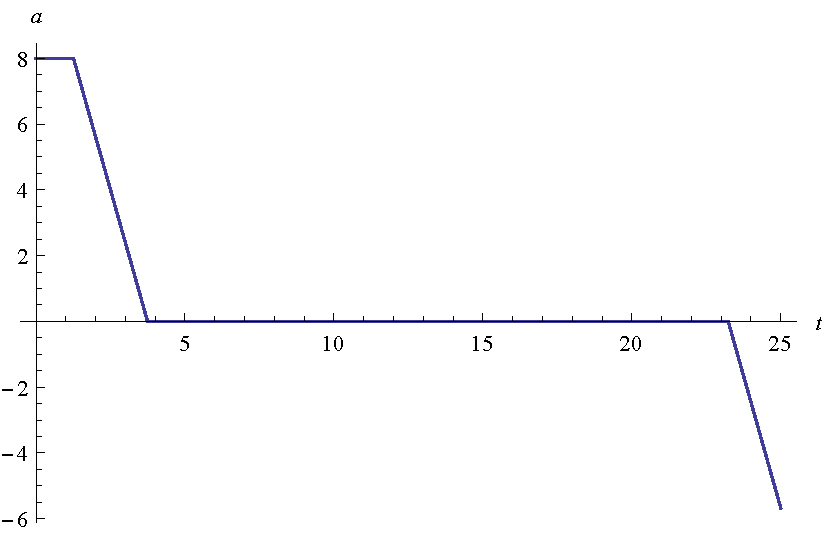
\includegraphics[width=9cm]{figures/uopt/a.pdf}
\caption{最大加速度约束下加速度仿真结果}
\label{fig:amax:a}
\end{figure}
\begin{figure}[htbp]
\centering
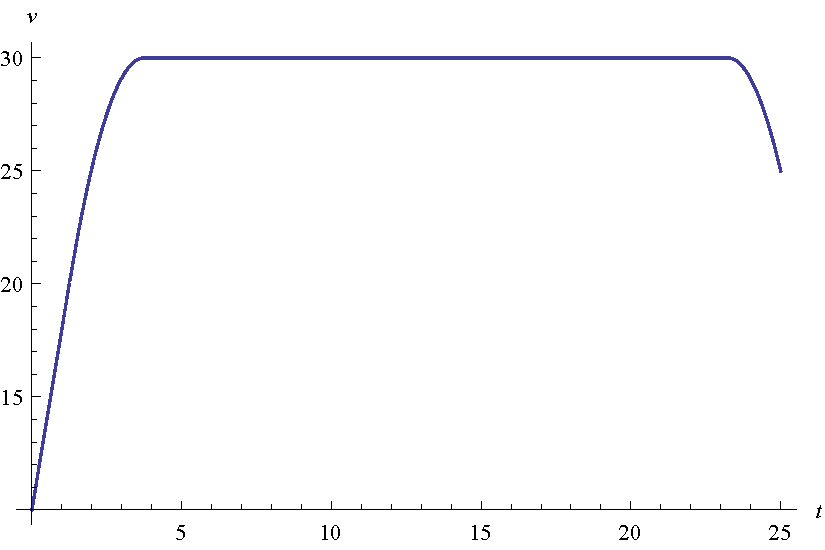
\includegraphics[width=9cm]{figures/uopt/v.pdf}
\caption{最大加速度约束下速度仿真结果}
\label{fig:amax:v}
\end{figure}

\subsection{双边加速度约束的简化问题}
考虑最大、最小加速度(最大减速度)都受限制的情况。与前一节的单边加速度受限情况相比,多出来最后一段以最大减速度减速的\textbf{匀减速段}。其中匀加速段和变加速段的系统状态与控制量仍可设为上一节的形式,分别如式\eqref{eq:amax:ea1}---\eqref{eq:amax:ea3}与式\eqref{eq:amax:ca1}---\eqref{eq:amax:ca3}。匀减速段的加速度、速度和位移设为($0\leq t\leq t_\mathrm{e}$)
\begin{gather}
u_\mathrm{e}(t)=u_{\min},\\
v_\mathrm{e}(t)=u_{\min}(t-t_\mathrm{e})+v_\mathrm{d},\\
p_\mathrm{e}(t)=\frac12 u_{\min}t^2+(v_\mathrm{d}-u_{\min}t_\mathrm{e})t.\\
\end{gather}
这里用到了$v_\mathrm{e}(t_e)=v_\mathrm{d}$和$p_\mathrm{e}(0)=0$的条件。根据整体位移量,速度和加速度的连续性可列出方程,
\begin{gather}
u_\mathrm{c}(t_\mathrm{c})=u_{\min},\label{eq:amin:1}\\
v_\mathrm{c}(0)=u_{\max}t_\mathrm{a}+v_0,\\
v_\mathrm{c}(t_\mathrm{c})=v_\mathrm{d}-u_{\min}t_\mathrm{e},\\
v_\mathrm{c}(-\frac{u_{\max}}{a})=-\frac12\frac{u_{\max}^2}{a}+c=v_\mathrm{max},\\
p_\mathrm{c}(t_\mathrm{c})+p_\mathrm{a}(t_\mathrm{a})+p_\mathrm{e}(t_\mathrm{e})+v_\mathrm{m}(t_\mathrm{m}-t_\mathrm{e}-t_\mathrm{a}-t_\mathrm{c})=L.\label{eq:amin:5}
\end{gather}
上述五个方程构成方程组,可解出五个参数$a,c,t_\mathrm{e},t_\mathrm{a},t_\mathrm{c}$。

对这种情况也给出一个具体算例,仿真参数如表\ref{tab:amin:param}。解方程式\eqref{eq:amin:1}---\eqref{eq:amin:5},得到如下两组实数解:
\[a = -5.19134,\ c = 23.8359,\ t_\mathrm{a} = 1.72949,\ t_\mathrm{c} = 2.11891,\ t_\mathrm{e} = 1.37772\]
和
\[a = 5.19134,\ c = 36.1641,\ t_\mathrm{a} = 3.27051,\ t_\mathrm{c} = -2.11891,\ t_\mathrm{e} = 1.95561\]
其中第二组解$t_\mathrm{c}<0$,舍弃,第一组解确定的加速度和速度分别如图\ref{fig:amin:ma}和图\ref{fig:amin:mv}。经检验,通过的位移确实为$L$。
\begin{table}[htbp]
\centering
\caption{最大加速度约束仿真实验参数}
\label{tab:amin:param}
\begin{tabular}{lll}
\toprule[1.5pt]
参数符号 & 参数含义 & 参数值 \\
\midrule[1pt]
$p_0$ & 初始位移 & $0$ \\
$L$($p_\mathrm{m}$) & 控制区长度(终点位移) & $\SI{720.0}{m}$ \\
$v_0$ & 初速度 & $\SI{10.0}{m\per s}$ \\
$v_\mathrm{d}$ & 期望速度 & $\SI{25.0}{m\per s}$ \\
$t_0$ & 初始时刻 & $0$ \\
$t_\mathrm{m}$ & 到达路口时刻 & $\SI{25.0}{s}$ \\
$v_{\max}$ & 最大速度限制 & $\SI{30.0}{m\per s}$ \\
$u_{\max}$ & 最大加速度限制 & $\SI{8}{m\per s\square}$ \\
$u_{\min}$ & 最大减速度限制 & $-\SI{3}{m\per s\square}$ \\
\bottomrule[1.5pt]
\end{tabular}
\end{table}

\begin{figure}[htbp]
\centering
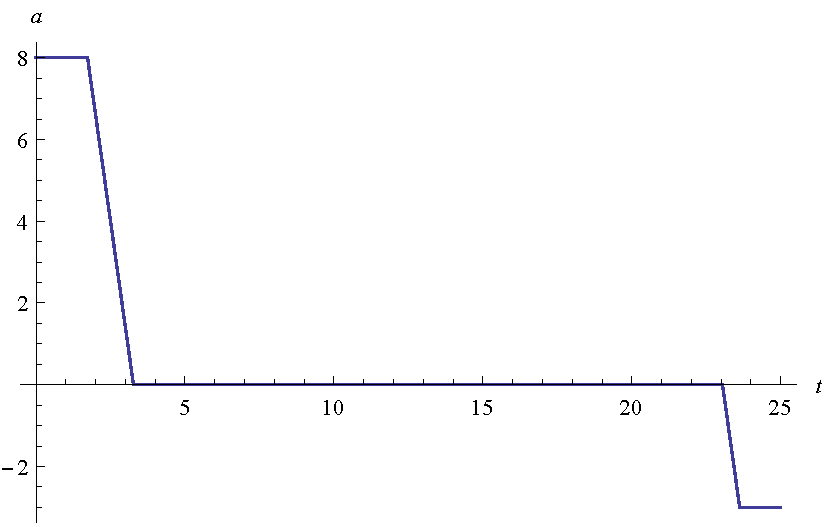
\includegraphics[width=9cm]{figures/uopt/ma.pdf}
\caption{最大最小加速度约束下加速度仿真结果}
\label{fig:amin:ma}
\end{figure}
\begin{figure}[htbp]
\centering
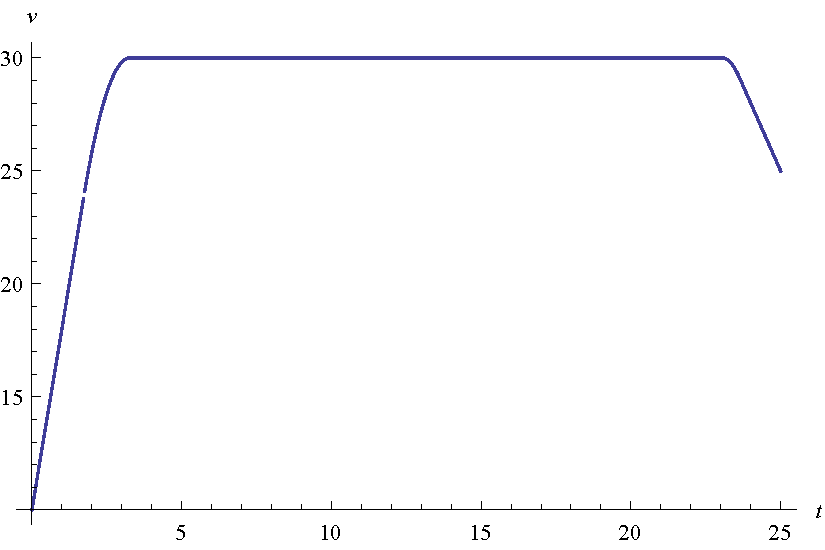
\includegraphics[width=9cm]{figures/uopt/mv.pdf}
\caption{最大最小加速度约束下速度仿真结果}
\label{fig:amin:mv}
\end{figure}

\section{总结}
至此,文章给出了在$t_\mathrm{m}$给定的情况下,存在各种约束时的最优控制求解方法。